\documentclass[11pt,a4paper]{article}
\usepackage[utf8]{inputenc}
\usepackage[T1]{fontenc}
\usepackage{lmodern}
\usepackage[spanish,es-tabla,es-nodecimaldot,es-noquoting]{babel}
\spanishplainpercent
\usepackage[a4paper,margin=2.4cm]{geometry}
\usepackage{amsmath,amssymb,graphicx,booktabs,float,xcolor,caption,listings,array}
\usepackage[output-decimal-marker={,},group-separator={\,},group-minimum-digits=4,
            exponent-product=\times,separate-uncertainty=true,range-phrase={--}]{siunitx}
\usepackage[hidelinks]{hyperref}
\DeclareUnicodeCharacter{2080}{\ensuremath{_0}}\DeclareUnicodeCharacter{2081}{\ensuremath{_1}}
\DeclareUnicodeCharacter{2082}{\ensuremath{_2}}\DeclareUnicodeCharacter{2083}{\ensuremath{_3}}
\DeclareUnicodeCharacter{2070}{\ensuremath{^0}}\DeclareUnicodeCharacter{00B9}{\ensuremath{^1}}
\DeclareUnicodeCharacter{2074}{\ensuremath{^4}}\DeclareUnicodeCharacter{2075}{\ensuremath{^5}}
\DeclareUnicodeCharacter{2076}{\ensuremath{^6}}\DeclareUnicodeCharacter{207B}{\ensuremath{^-}}
\DeclareUnicodeCharacter{03B1}{\ensuremath{\alpha}}\DeclareUnicodeCharacter{03B2}{\ensuremath{\beta}}
\DeclareUnicodeCharacter{03B3}{\ensuremath{\gamma}}\DeclareUnicodeCharacter{03B4}{\ensuremath{\delta}}
\DeclareUnicodeCharacter{03B5}{\ensuremath{\varepsilon}}\DeclareUnicodeCharacter{03B8}{\ensuremath{\theta}}
\DeclareUnicodeCharacter{03BB}{\ensuremath{\lambda}}\DeclareUnicodeCharacter{03BC}{\ensuremath{\mu}}
\DeclareUnicodeCharacter{03BD}{\ensuremath{\nu}}\DeclareUnicodeCharacter{03C0}{\ensuremath{\pi}}
\DeclareUnicodeCharacter{03C1}{\ensuremath{\rho}}\DeclareUnicodeCharacter{03C3}{\ensuremath{\sigma}}
\DeclareUnicodeCharacter{03C4}{\ensuremath{\tau}}\DeclareUnicodeCharacter{03C6}{\ensuremath{\phi}}
\DeclareUnicodeCharacter{03C7}{\ensuremath{\chi}}\DeclareUnicodeCharacter{03C9}{\ensuremath{\omega}}
\DeclareUnicodeCharacter{0394}{\ensuremath{\Delta}}\DeclareUnicodeCharacter{03A3}{\ensuremath{\Sigma}}
\DeclareUnicodeCharacter{2212}{\ensuremath{-}}\DeclareUnicodeCharacter{2248}{\ensuremath{\approx}}
\DeclareUnicodeCharacter{2264}{\ensuremath{\le}}\DeclareUnicodeCharacter{2265}{\ensuremath{\ge}}
\DeclareUnicodeCharacter{2192}{\ensuremath{\to}}\DeclareUnicodeCharacter{27E8}{\ensuremath{\langle}}
\DeclareUnicodeCharacter{27E9}{\ensuremath{\rangle}}\DeclareUnicodeCharacter{2032}{\ensuremath{'}}
\DeclareUnicodeCharacter{2033}{\ensuremath{''}}
\captionsetup{font=small,labelfont=bf}
\setlength{\parskip}{4pt}
\definecolor{fondo}{HTML}{F6F6F4}
\lstset{language=Python,basicstyle=\ttfamily\scriptsize,backgroundcolor=\color{fondo},frame=single,
  rulecolor=\color{gray!40},breaklines=true,columns=fullflexible,keepspaces=true,showstringspaces=false,
  numbers=left,numberstyle=\tiny\color{gray},keywordstyle=\color{blue!60!black}\bfseries,
  commentstyle=\color{green!40!black}\itshape,stringstyle=\color{red!50!black},
  escapeinside={(*@}{@*)}}

\usepackage{longtable}
\title{\textbf{Proyecto 19. Acelerador lineal}\\[4pt]\large Aceleradores --- Nivel III}
\author{Jaime A. Betancourt\\\small Herramientas Computacionales para la Física --- Proyectos avanzados con Python}
\date{\today}
\begin{document}
\maketitle
\begin{abstract}
Se modela un acelerador lineal de tubos de deriva para protones a \num{352.2}~MHz en el que cada cavidad aporta
$\Delta E=qV\cos\phi$, de modo que tras $N$ cavidades $E_N=E_0+\sum qV_i\cos\phi_i$. Se diseñan las celdas para la partícula
síncrona ($L_n=\beta_n\lambda$): con $qV=\num{1.0}$~MeV y $\phi_s=-30°$ se pasa de \num{3} a \num{50}~MeV en 55 celdas y \num{10.59}~m. Siguiendo un
paquete de \num{3000} partículas con dispersión de fase y energía se estudia la estabilidad de fase: con $\phi_s=-30°$ el \num{99.3}\,\% del
paquete permanece agrupado y realiza oscilaciones de sincrotrón cuyo avance de fase coincide con la teoría de pequeña amplitud,
mientras que en la cresta ($\phi_s=0$) solo el \num{24.1}\,\% llega a la energía final. Se estudian además el efecto de un error en la
frecuencia del RF y el caso de los electrones, que viajan a $\beta\simeq1$ y no tienen oscilaciones de fase.
\end{abstract}
\tableofcontents
\newpage
\section{Introducción}

Un acelerador lineal (linac) acelera partículas haciéndolas atravesar una sucesión de cavidades o huecos en los que un campo
eléctrico de radiofrecuencia las empuja. Para que el campo empuje siempre en el sentido correcto, la partícula debe llegar a
cada hueco en la misma fase del RF: mientras está en los tubos de deriva, apantallada, el campo cambia de signo. Por eso las
celdas deben alargarse a medida que la partícula se acelera. Los linacs son los inyectores de casi todos los grandes
aceleradores, se usan en radioterapia (electrones de 6--18~MeV) y son la base de las fuentes de espalación. Este proyecto
estudia el diseño de un linac de protones, la dinámica longitudinal de un paquete y la estabilidad de fase.

\section{Objetivos}

\begin{enumerate}
\item Implementar el modelo de aceleración por cavidades $\Delta E=qV\cos\phi$ y $E_N=E_0+\sum qV_i\cos\phi_i$.
\item Diseñar las longitudes de las celdas para la partícula síncrona.
\item Estudiar el efecto de la fase y la sincronización sobre un paquete de partículas.
\item Verificar la teoría de las oscilaciones de sincrotrón y comparar protones con electrones.
\end{enumerate}

\section{Fundamento físico}

En el hueco $i$ la partícula gana $\Delta E_i=qV\cos\phi_i$, donde $\phi_i$ es la fase del RF al cruzarlo ($\phi=0$ en la cresta).
Para que la partícula síncrona llegue a cada hueco con la misma fase $\phi_s$, la distancia entre huecos debe recorrerse en un
periodo del RF: $L_n=\beta_n\lambda$, con $\lambda=c/f=\num{85.1}$~cm (estructura de Alvarez). Una partícula que llega con un pequeño
retraso $\Delta\phi$ recibe una energía distinta; si $\phi_s<0$ (la partícula llega antes de la cresta, en el flanco de subida del
voltaje), la que llega tarde gana \emph{más} energía, va más rápida y se adelanta: la fase es estable. Linealizando,
\begin{equation}
\frac{d\Delta\phi}{dn}=-\frac{2\pi\,\Delta W}{mc^2\beta^2\gamma^3},\qquad \frac{d\Delta W}{dn}=-qV\sin\phi_s\,\Delta\phi, \label{eq:lin}
\end{equation}
que describe oscilaciones (de sincrotrón) con avance de fase por celda
\begin{equation}
\mu^2=\frac{2\pi qV(-\sin\phi_s)}{mc^2\beta^2\gamma^3}. \label{eq:mu}
\end{equation}
Con $\phi_s>0$ la partícula retrasada gana menos energía y se retrasa aún más: inestable. El precio de la estabilidad es una
ganancia menor que la máxima ($\cos\phi_s<1$). Para amplitudes grandes la dinámica es la de un péndulo, con una región estable
(separatriz) que va de $-\phi_s$ a una fase $\phi_2\approx2\phi_s$. Al acelerarse, $\mu$ disminuye y la amplitud de fase se
amortigua adiabáticamente (como $(\beta\gamma)^{-3/4}$).

Los electrones de más de unos MeV ya viajan a $\beta\approx1$: su fase no cambia, no hay oscilaciones y pueden acelerarse en la cresta.

\section{Modelo matemático}

Cada partícula se describe por $(T_i,\phi_i)$ a la entrada del hueco $i$. El mapa de una celda es
\begin{align}
T_{i+1}&=T_i+qV\cos\phi_i,\\
\phi_{i+1}&=\phi_i+\omega\frac{L_i}{\beta(T_{i+1})c}-2\pi ,
\end{align}
donde $L_i$ es la celda de diseño. Para la partícula síncrona el segundo término es exactamente $2\pi$ y su fase no cambia. Un
error relativo $\epsilon$ en la frecuencia se modela sustituyendo $\omega$ por $\omega(1+\epsilon)$. Parámetros: $f=\num{352.2}$~MHz,
$qV=\num{1.0}$~MeV por hueco, $T$ de \num{3} a \num{50}~MeV.

\section{Método numérico}

El diseño se construye iterando la ecuación de la energía para la partícula síncrona y calculando $\beta$ al final de cada
celda. El mapa se aplica de forma vectorizada a \num{3000} partículas con $\Delta\phi_0\sim\mathcal N(0,15°)$ y
$\Delta T_0/T_0\sim\mathcal N(0;0{,}5~\%)$. El avance de fase simulado se mide a partir de los cruces por cero de $\Delta\phi$ de
una partícula con amplitud inicial de 3° (medio periodo entre cruces consecutivos) y se compara con~\eqref{eq:mu}.

\section{Implementación computacional}

\texttt{src/modelo.py} contiene $\beta(T)$, el diseño de celdas, el seguimiento del paquete, el avance de fase teórico y la
aceptancia de fase. \texttt{src/simulacion.py} produce el diseño, la tabla de estabilidad, las oscilaciones, el estudio del error
de frecuencia y el caso de los electrones; los paquetes completos se guardan en \texttt{datos/paquete\_fase*.npz}.

\section{Resultados}

\subsection{Diseño}
Con $\phi_s=-30°$ la partícula síncrona gana \num{0.866}~MeV por hueco y necesita 55 celdas y \num{10.59}~m para ir de \num{3} a \num{50}~MeV
(gradiente medio \num{4.44}~MeV/m). Las celdas crecen de \num{7.7} a \num{26.9}~cm, siguiendo $\beta\lambda$ (figura~\ref{fig:fig01_diseno}).
Con $\phi_s=-60°$ harían falta 94 celdas y en la cresta solo 47: la estabilidad cuesta longitud.

\begin{figure}[H]
\centering
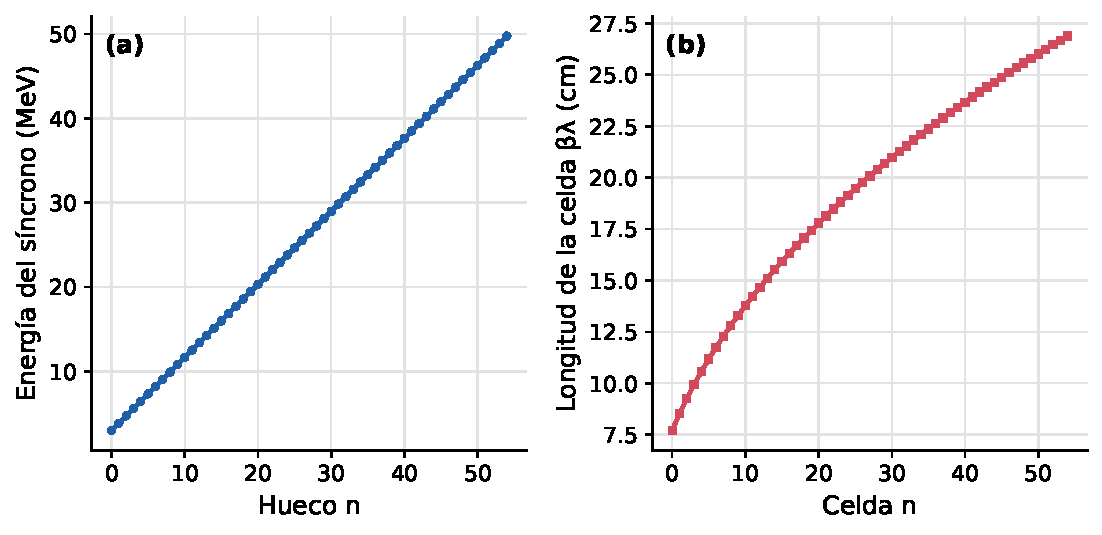
\includegraphics[width=0.95\linewidth]{../figuras/fig01_diseno.pdf}
\caption{(a) Energía de la partícula síncrona en cada hueco y (b) longitud de las celdas del linac ($\phi_s=-30°$).}
\label{fig:fig01_diseno}
\end{figure}

\subsection{Estabilidad de fase}
La figura~\ref{fig:fig02_espacio_fases} muestra el paquete en el espacio $(\Delta\phi,\Delta W)$. Con $\phi_s=-30°$ las partículas giran
alrededor de la síncrona: la dispersión de fase se reduce de \num{15.0}° a \num{5.3}° (amortiguamiento adiabático) a cambio de una dispersión
de energía de \num{282}~keV, y el \num{99.3}\,\% permanece agrupado. La tabla~\ref{tab:estabilidad} compara las fases síncronas: con $-60°$ se conserva
el \num{100.0}\,\% y con $-15°$ el \num{88.9}\,\% (la separatriz es más estrecha). En la cresta ($\phi_s=0$) no hay fuerza restauradora y solo el \num{24.1}\,\% del paquete
llega a la energía final. Con $\phi_s=+30°$ el síncrono de diseño es inestable, pero ocurre algo instructivo: parte del paquete migra a la
fase estable simétrica $-30°$, que da la misma ganancia $\cos(\pm30°)$; el \num{45.9}\,\% llega a la energía final con una fase media de \num{-18}°.

\begin{table}[H]
\centering
\caption{Estabilidad de un paquete ($\sigma_\phi=15°$, $\sigma_W/W=0{,}5~\%$ iniciales) para distintas fases síncronas; cada fase tiene su propio diseño de celdas. ``Energía final'': fracción que llega a la energía de diseño $\pm1$~MeV.}
\label{tab:estabilidad}
\small
\begin{tabular}{lccccc}
\toprule
$\phi_s$ (°) & Celdas & $|\Delta\phi|<60°$ & Energía final & $\sigma_\phi$ final (°) & $\sigma_W$ final (keV) \\
\midrule
-60 & 94 & \num{100.0}\,\% & \num{99.6}\,\% & \num{7.4} & \num{155} \\
-30 & 55 & \num{99.3}\,\% & \num{99.2}\,\% & \num{5.3} & \num{282} \\
-15 & 49 & \num{88.9}\,\% & \num{88.9}\,\% & \num{5.0} & \num{122} \\
0 & 47 & \num{26.8}\,\% & \num{24.1}\,\% & \num{14.4} & \num{457} \\
+30 & 55 & \num{41.4}\,\% & \num{45.9}\,\% & \num{6.8} & \num{547} \\
\bottomrule
\end{tabular}
\end{table}


\begin{figure}[H]
\centering
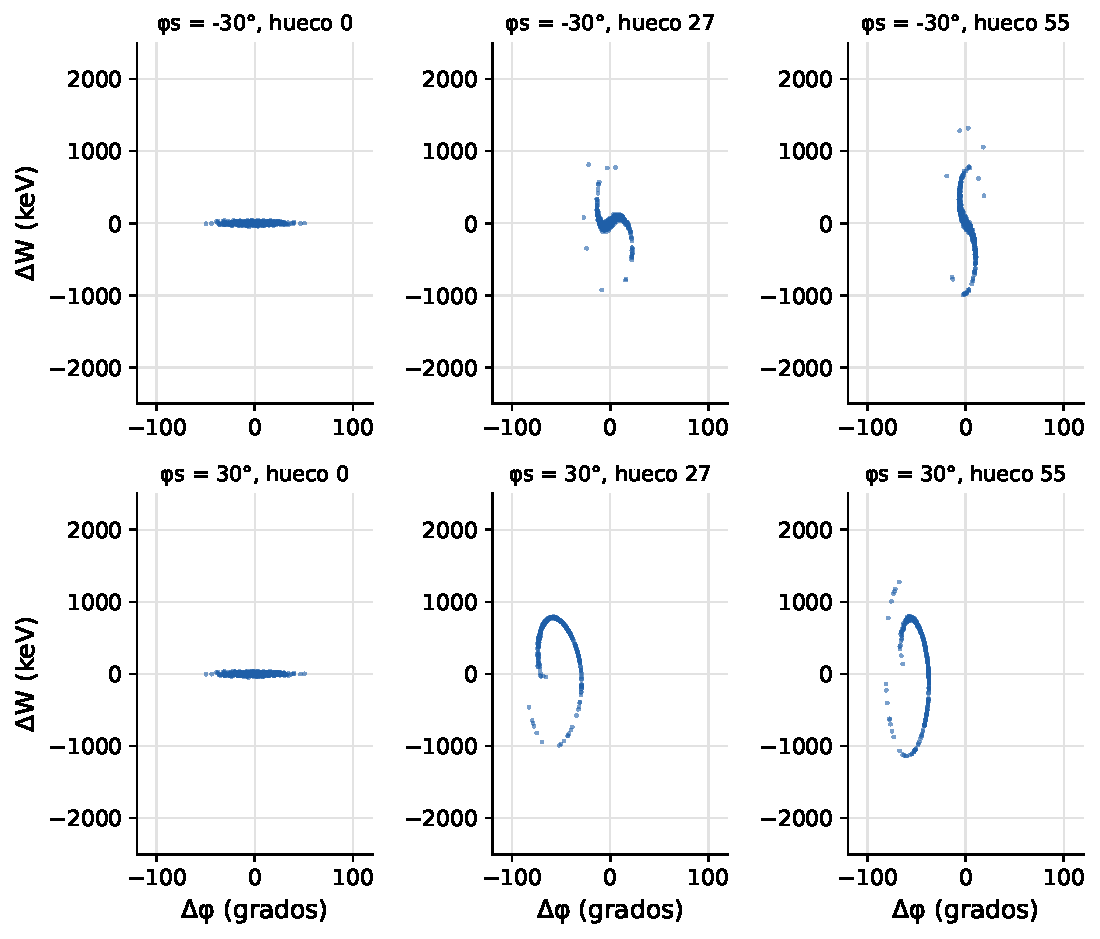
\includegraphics[width=0.95\linewidth]{../figuras/fig02_espacio_fases.pdf}
\caption{Espacio de fases longitudinal del paquete al principio, en la mitad y al final del linac para $\phi_s=-30°$ (arriba, estable) y $\phi_s=+30°$ (abajo).}
\label{fig:fig02_espacio_fases}
\end{figure}

\subsection{Oscilaciones de sincrotrón}
Una partícula con 3° de desfase inicial oscila alrededor de la síncrona (figura~\ref{fig:fig03_sincrotron}). El avance de fase medido en la
primera semioscilación es \num{25.7}°/celda, frente a \num{26.4}° de la ecuación~\eqref{eq:mu}; a lo largo del linac el avance teórico baja de
\num{41.4}° a \num{9.8}° por celda y la simulación lo sigue. La amplitud se reduce de \num{3.0}° a \num{1.39}°: es el amortiguamiento adiabático, del orden de la ley
$(\beta\gamma)^{-3/4}$ (que predice un factor 0,35 entre 3 y 50~MeV; el valor simulado, 0,46, incluye la fase de la oscilación en la
última celda).

\begin{figure}[H]
\centering
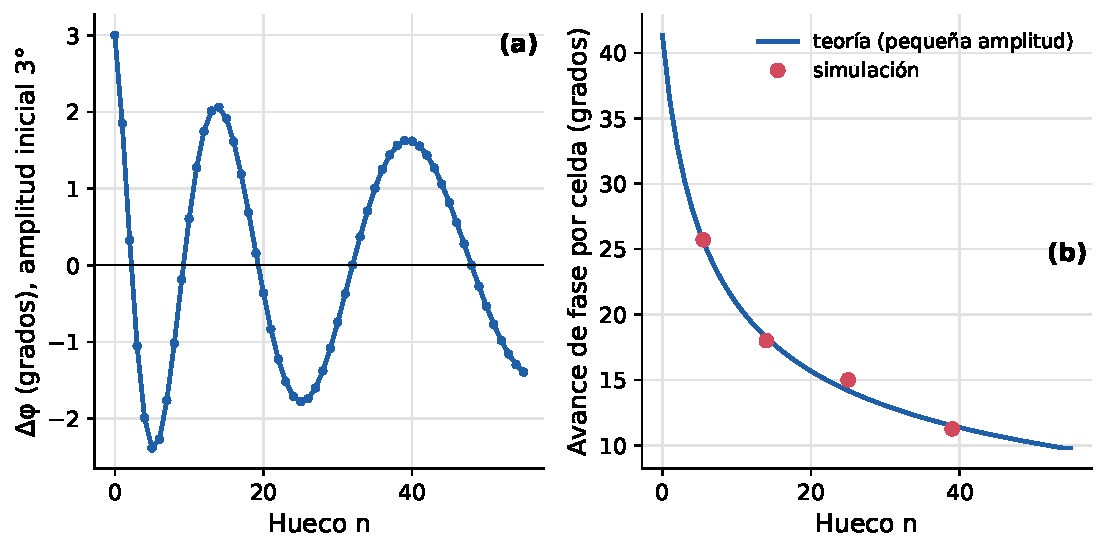
\includegraphics[width=0.95\linewidth]{../figuras/fig03_sincrotron.pdf}
\caption{(a) Oscilación de fase de una partícula con 3° de desfase inicial. (b) Avance de fase por celda: teoría de pequeña amplitud y simulación.}
\label{fig:fig03_sincrotron}
\end{figure}

\subsection{Sincronización y electrones}
Un error en la frecuencia hace que el paquete llegue cada vez a una fase distinta; la estabilidad de fase lo compensa desplazando el
paquete hacia una nueva fase de equilibrio (tabla~\ref{tab:errorf}): con un 1~\% de error el paquete se desplaza \num{5.1}° y llega a \num{51.69}~MeV,
conservando el \num{98.1}\,\% de las partículas; con un 2~\% se conserva el \num{94.5}\,\% y con un 4~\% solo el \num{55.5}\,\% (figura~\ref{fig:fig04_estabilidad_electrones}(b)).
Los electrones de \num{10}~MeV inyectados en 60 celdas de longitud $\lambda$ alcanzan \num{69.92}~MeV en la cresta, y su fase deriva solo \num{3.6}° en todo el
linac: sin oscilaciones, la energía final depende directamente de la fase de inyección ($\cos40°$: \num{53.55}~MeV), figura~\ref{fig:fig04_estabilidad_electrones}(c).

\begin{table}[H]
\centering
\caption{Efecto de un error relativo en la frecuencia del RF ($\phi_s=-30°$).}
\label{tab:errorf}
\small
\begin{tabular}{lccc}
\toprule
Error de frecuencia & Capturadas & $\langle T\rangle$ final (MeV) & Desplazamiento de fase (°) \\
\midrule
\num{0.0}\,\% & \num{99.3}\,\% & \num{50.64} & \num{0.6} \\
\num{0.2}\,\% & \num{99.0}\,\% & \num{50.86} & \num{1.4} \\
\num{0.5}\,\% & \num{99.0}\,\% & \num{51.18} & \num{2.9} \\
\num{1.0}\,\% & \num{98.1}\,\% & \num{51.69} & \num{5.1} \\
\num{2.0}\,\% & \num{94.5}\,\% & \num{52.66} & \num{7.4} \\
\num{4.0}\,\% & \num{55.5}\,\% & \num{55.50} & \num{10.7} \\
\bottomrule
\end{tabular}
\end{table}


\begin{figure}[H]
\centering
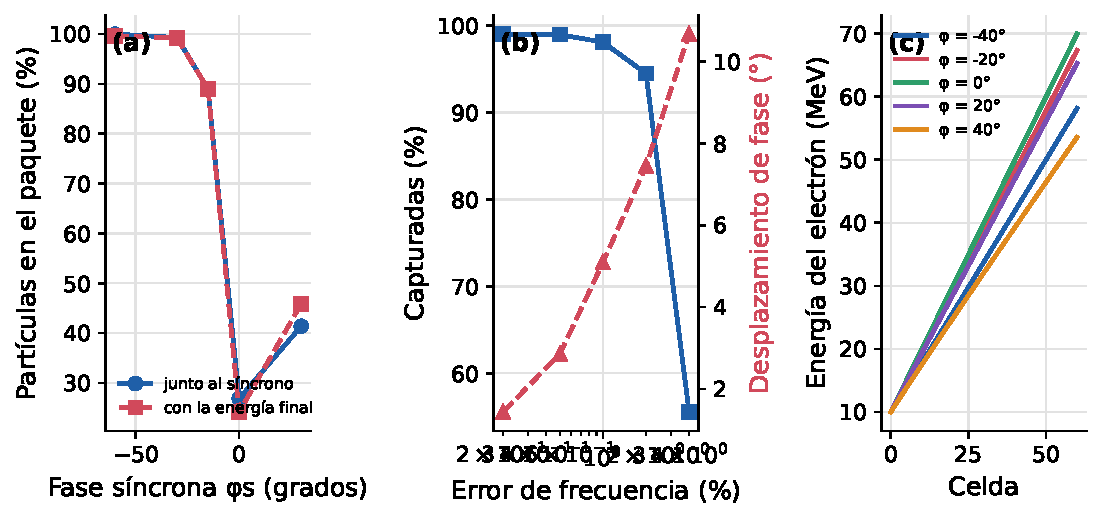
\includegraphics[width=0.95\linewidth]{../figuras/fig04_estabilidad_electrones.pdf}
\caption{(a) Fracción del paquete agrupada y fracción que llega a la energía final frente a la fase síncrona. (b) Efecto de un error de frecuencia. (c) Energía de electrones inyectados con distintas fases.}
\label{fig:fig04_estabilidad_electrones}
\end{figure}


\section{Análisis de incertidumbre y validación}

\begin{itemize}
\item \textbf{Ecuación de la guía:} la energía del síncrono reproduce exactamente $E_N=E_0+NqV\cos\phi_s$.
\item \textbf{Teoría lineal:} el avance de fase simulado coincide con~\eqref{eq:mu} dentro de la resolución de la medida (que usa un
      número entero de celdas por semioscilación).
\item \textbf{Comportamiento cualitativo:} estabilidad para $\phi_s<0$ e inestabilidad para $\phi_s>0$, como predice la teoría.
\item \textbf{Estadística:} con \num{3000} partículas, las fracciones tienen errores de $\sim1~\%$.
\item \textbf{Simplificaciones:} huecos de longitud nula (sin factor de tiempo de tránsito), voltaje constante en todas las celdas,
      sin dinámica transversal (en un linac real la focalización de fase desenfoca transversalmente y se compensa con cuadrupolos),
      sin carga espacial.
\end{itemize}

\section{Discusión}

La estabilidad de fase, descubierta por Veksler y McMillan en 1944--45, es la idea que hizo posibles los aceleradores modernos:
basta elegir la fase síncrona en el flanco adecuado del RF para que el paquete se mantenga unido de forma natural, aunque las partículas
tengan energías y fases ligeramente distintas. El mismo principio funciona en los sincrotrones. El proyecto muestra también el compromiso
de diseño: una fase síncrona más negativa da una región estable más grande pero menos ganancia por celda y por tanto un linac más largo.
Para electrones relativistas el problema es distinto: no hay oscilaciones, la fase se fija en la inyección y el agrupamiento se hace antes,
en un ``buncher''. Por eso los linacs médicos de electrones son compactos y trabajan cerca de la cresta.

\section{Conclusiones}

\begin{itemize}
\item Linac de protones de \num{3} a \num{50}~MeV con \num{1.0}~MV por hueco y $\phi_s=-30°$: 55 celdas, \num{10.59}~m, celdas de \num{7.7} a \num{26.9}~cm.
\item Con $\phi_s=-30°$ el paquete es estable (\num{99.3}\,\% agrupado); en la cresta solo llega a la energía final el \num{24.1}\,\%.
\item El avance de fase de las oscilaciones de sincrotrón sigue la teoría lineal y la amplitud se amortigua adiabáticamente.
\item La estabilidad de fase tolera errores de frecuencia de hasta $\sim2~\%$; los electrones no tienen oscilaciones de fase.
\end{itemize}


\section{Reproducibilidad y archivos}
Todos los resultados de este informe se regeneran desde la carpeta del proyecto con
\begin{verbatim}
python3 src/simulacion.py     # genera los datos (datos/) y el analisis (resultados/)
python3 src/graficas.py       # genera las figuras (figuras/, PNG y PDF)
python3 src/informe.py        # escribe y compila este informe y la presentacion
\end{verbatim}
Las semillas de los generadores aleatorios están fijadas en \texttt{datos/parametros.json}, de modo que
la ejecución repetida produce exactamente los mismos números. Archivos del proyecto:
{\small
\begin{longtable}{ll}
\toprule
Archivo & Tamaño \\
\midrule
\texttt{datos/fase\_media\_error0.0.npy} & 0.4 kB \\
\texttt{datos/fase\_media\_error0.002.npy} & 0.4 kB \\
\texttt{datos/fase\_media\_error0.005.npy} & 0.4 kB \\
\texttt{datos/fase\_media\_error0.01.npy} & 0.4 kB \\
\texttt{datos/fase\_media\_error0.02.npy} & 0.4 kB \\
\texttt{datos/fase\_media\_error0.04.npy} & 0.4 kB \\
\texttt{datos/paquete\_fase-15.npz} & 300.1 kB \\
\texttt{datos/paquete\_fase-30.npz} & 334.7 kB \\
\texttt{datos/paquete\_fase-60.npz} & 568.0 kB \\
\texttt{datos/paquete\_fase0.npz} & 286.5 kB \\
\texttt{datos/paquete\_fase30.npz} & 326.4 kB \\
\texttt{datos/parametros.json} & 0.4 kB \\
\texttt{src/graficas.py} & 3.4 kB \\
\texttt{src/informe.py} & 16.8 kB \\
\texttt{src/modelo.py} & 2.6 kB \\
\texttt{src/simulacion.py} & 5.4 kB \\
\texttt{resultados/avance\_sincrotron.csv} & 0.1 kB \\
\texttt{resultados/celdas\_vs\_fase.csv} & 0.1 kB \\
\texttt{resultados/diseno\_celdas.csv} & 1.6 kB \\
\texttt{resultados/electrones.csv} & 5.1 kB \\
\texttt{resultados/error\_frecuencia.csv} & 0.2 kB \\
\texttt{resultados/estabilidad\_fase.csv} & 0.5 kB \\
\texttt{resultados/oscilacion\_pequena.csv} & 1.2 kB \\
\texttt{resultados/resumen.json} & 0.6 kB \\
\texttt{figuras/fig01\_diseno.pdf} & 20.3 kB \\
\texttt{figuras/fig01\_diseno.png} & 85.7 kB \\
\texttt{figuras/fig02\_espacio\_fases.pdf} & 77.6 kB \\
\texttt{figuras/fig02\_espacio\_fases.png} & 126.2 kB \\
\texttt{figuras/fig03\_sincrotron.pdf} & 21.2 kB \\
\texttt{figuras/fig03\_sincrotron.png} & 110.7 kB \\
\texttt{figuras/fig04\_estabilidad\_electrones.pdf} & 28.7 kB \\
\texttt{figuras/fig04\_estabilidad\_electrones.png} & 183.4 kB \\
\bottomrule
\end{longtable}}

\begin{thebibliography}{99}
\bibitem{wangler} T.~P. Wangler, \emph{RF Linear Accelerators}, 2.ª ed., Wiley-VCH (2008), caps. 4 y 6.
\bibitem{wille} K. Wille, \emph{The Physics of Particle Accelerators}, Oxford University Press (2000), cap. 4.
\bibitem{veksler} V.~I. Veksler, ``A new method of acceleration of relativistic particles'', \emph{J. Phys. USSR} \textbf{9} (1945) 153; E.~M. McMillan, \emph{Phys. Rev.} \textbf{68} (1945) 143.
\bibitem{cas} CERN Accelerator School, \emph{RF for Accelerators}, CERN-2011-007 (2011).
\end{thebibliography}
\appendix
\section{Código fuente}\label{sec:codigo}
A continuación se incluye el código completo del proyecto. Los módulos comunes (\texttt{comun/}) se documentan en el README general de la carpeta \texttt{Computacion-fisica}.
\subsection*{\texttt{src/graficas.py}}\addcontentsline{toc}{subsection}{\texttt{src/graficas.py}}
\lstinputlisting{codigo/graficas.py}
\subsection*{\texttt{src/informe.py}}\addcontentsline{toc}{subsection}{\texttt{src/informe.py}}
\lstinputlisting{codigo/informe.py}
\subsection*{\texttt{src/modelo.py}}\addcontentsline{toc}{subsection}{\texttt{src/modelo.py}}
\lstinputlisting{codigo/modelo.py}
\subsection*{\texttt{src/simulacion.py}}\addcontentsline{toc}{subsection}{\texttt{src/simulacion.py}}
\lstinputlisting{codigo/simulacion.py}
\end{document}